\section{Evaluation}
\label{sec:evaluation}

\begin{figure}[tb]
	\centering
	\includegraphics[width=6cm]{../img/throughput_comparison}
	\caption{throughput comparison with and without I/O burst buffer}
	\label{throughput comparison}
\end{figure}

\begin{figure}[tb]
	\centering
	\includegraphics[width=6cm]{../img/cache_hit_rate_throughput}
	\caption{throughput comparison between each cache hit rate}
	\label{throughput cache rate}
\end{figure}

\begin{figure}[tb]
	\centering
	\includegraphics[width=6cm]{../img/maximum_throughput}
	\caption{maximum avaliable throughput}
	\label{maximum throughput}
\end{figure}

\begin{figure}[tb]
	\centering
	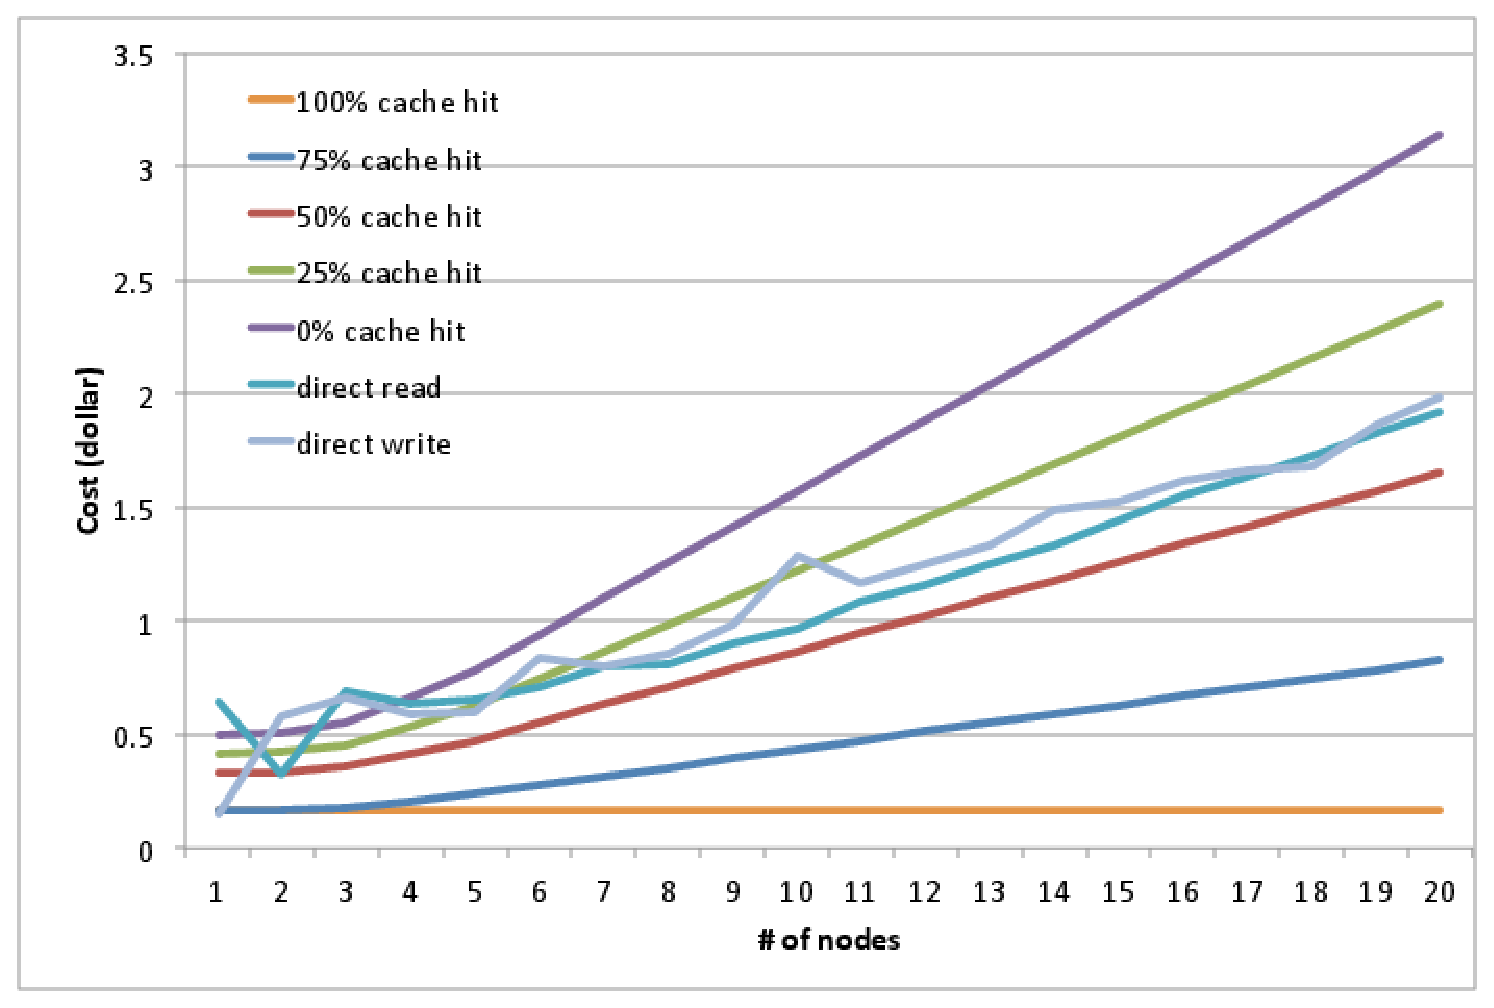
\includegraphics[width=6cm]{../img/cost}
	\caption{cost comparison}
	\label{cost}
\end{figure}

%\begin{figure}[tb]
%	\centering
%	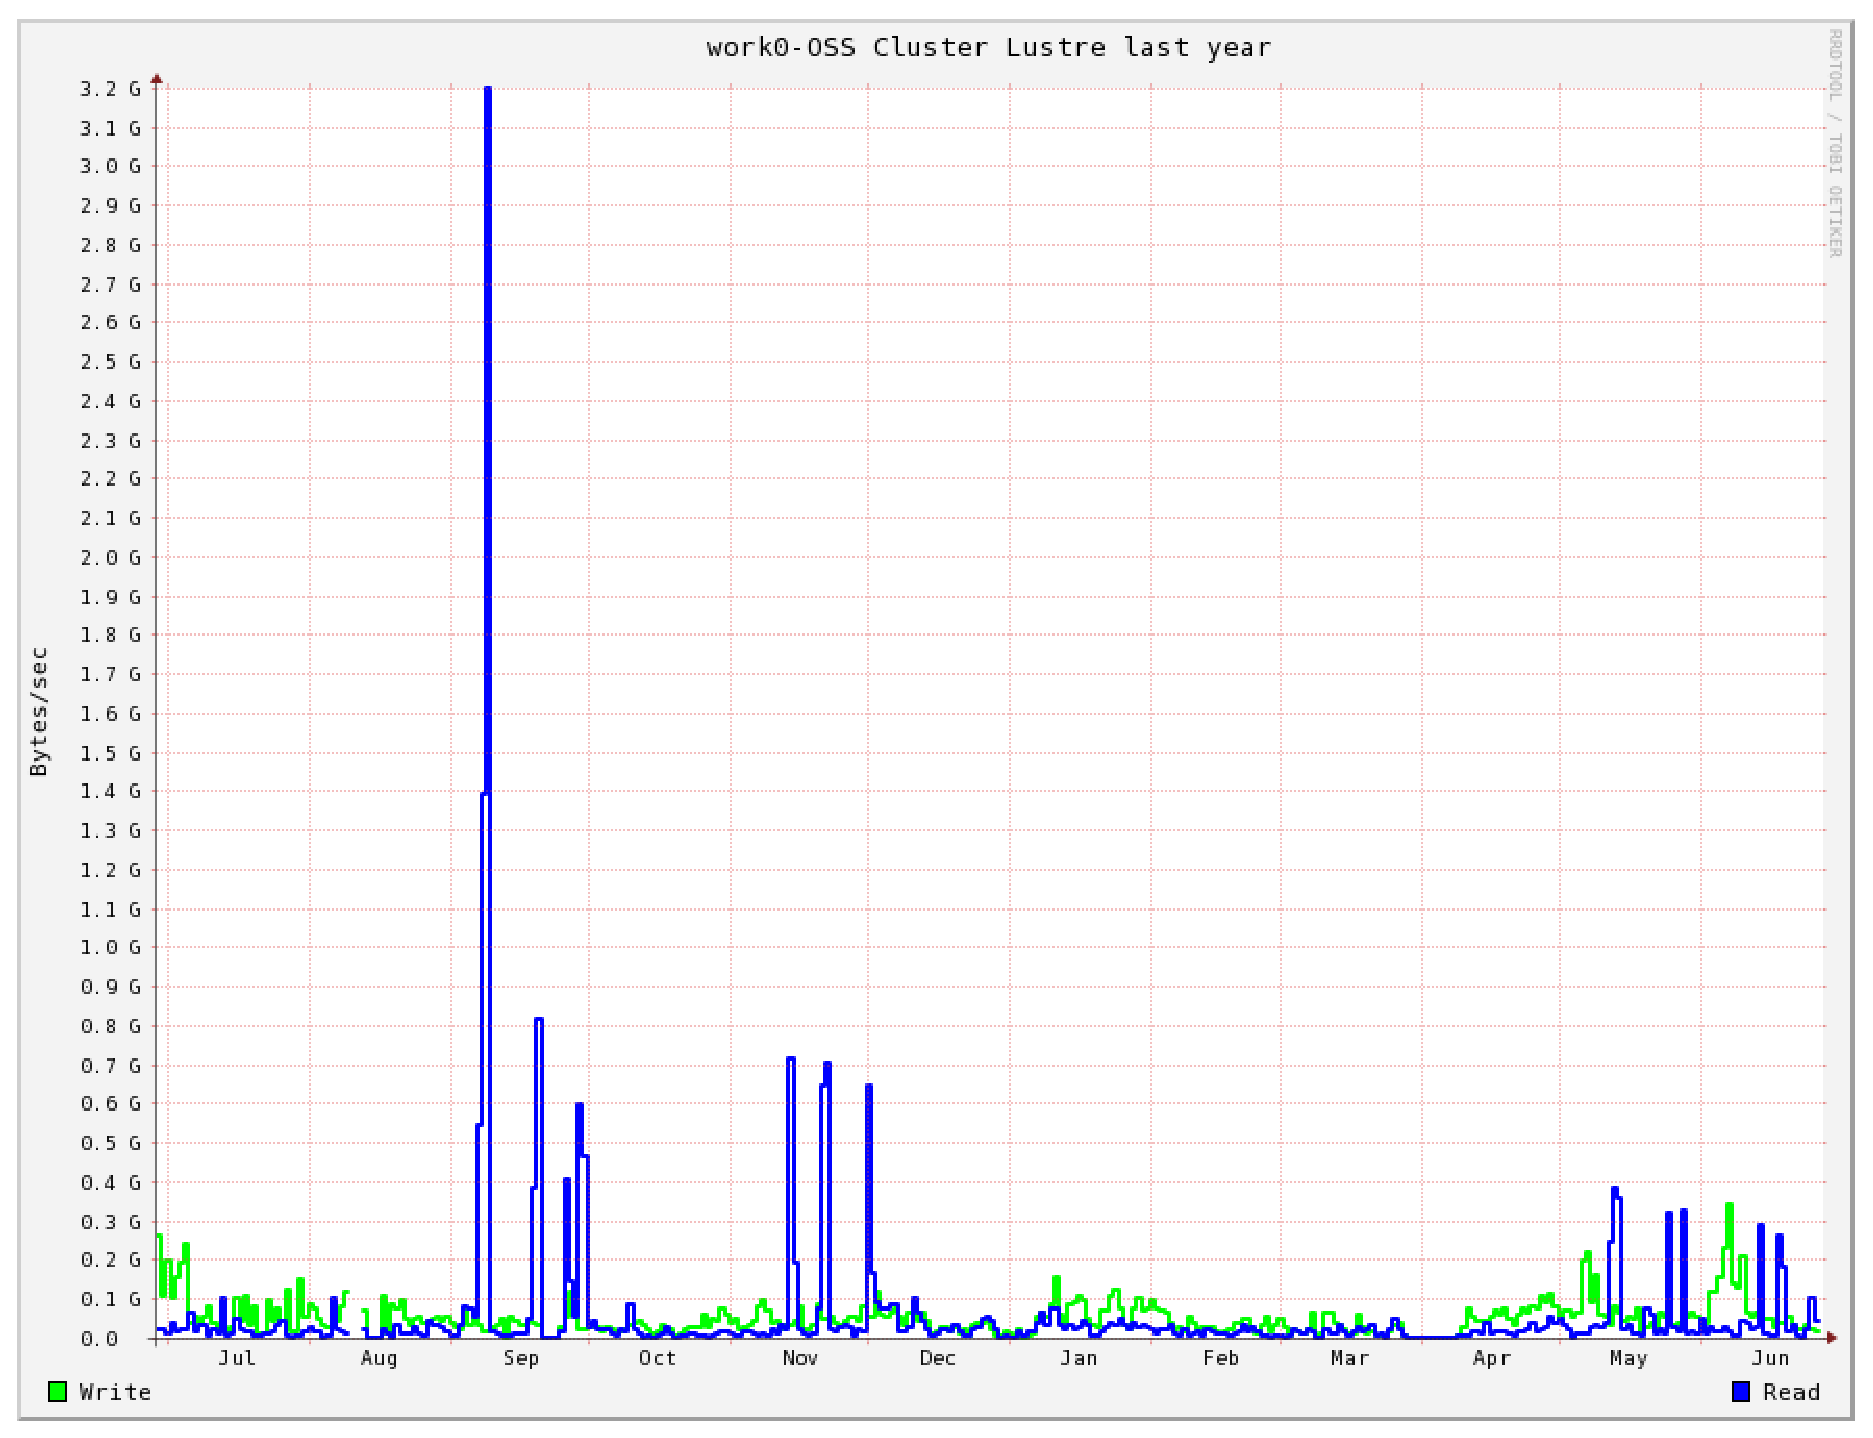
\includegraphics[width=6cm]{tsubamelustre}
%	\caption{TSUBAME Lustre workload}
%	\label{Lustre workload}
%\end{figure}
To evaluate how much federated systems with I/O burst buffers can improve I/O performance and the cost, 
we conduct several simulations based on preliminary performance data taken from several 
benchmarks on both our in-house cluster and Amazon EC2 in a Tokyo region in Section \ref{sec:motivation}.%, using
In the simulations, we assume that computing nodes running on one system read or write files on storage of the other system with the same I/O throghputs for both read and write operations.
We also assume an instance type of both the computing nodes and I/O burst buffer nodes is m3.xlarge provided by Amazon EC2.
We compare I/O throughputs and overall costs of a system using direct I/O with a system using I/O burst buffer by scaling out up to 20 computing nodes
under different cahch hit rate.
For read operations, the cache hit rate means percentage of data, which is read from buffer queues, to total read size. 
For write operations, the cache hit rate means percentage of data, which is  written to buffer queues before queue becomes full, to total write size.
%Consider we have up to 20 m3.xlarge computing nodes need to transfer data between two systems, 
%Since read and write throughput are the same when using caches on I/O burst buffers, read and write throughputs are equal to throghputs  between computing nodes and I/O nodes,  we use this throughput value for I/O throughput when use I/O burst buffer..
If read and write are completed via caches on I/O burst buffers
without accessing to remote storage, read and write throghputs become 
identical to throughputs between a compute node and I/O burst buffer nodes. 
%Thus, we use these throughputs for I/O throghputs
%m3.medium instance, which has a moderate Ethernet condition and one vcpu with 3.75GiB memory, and
%m3.xlarge instance, which has a high Ethernet condition and 8 vCPUs with 30GiB memory, run Amazon Linux AMI 2014.03.2(HVM) ( Fig.~\ref{throughput TSUBAME}, Fig.~\ref{throughput AMAZON to OURLAB}. Fig.~\ref{point to point connection AMAZON}, Fig.~\ref{point to point connection LAB} ).
%According to these data and definition described above, we use values defined below.

%\begin{center}
%\begin{tabular}[tb]{|c|c|}\hline
%	$D_2$&$E_1$\\\hline
%	8TB/s&1.08Gbit/s(135MB/s)\\\hline
	
%\end{tabular}
%\end{center}
%For throughput between two systems and inside system, from benchmark data, it shows it is hard to achieve a high throughput with only one nodes, and also there is a limit on maximum throughput between two systems and inside system.
%Although incresing nodes can increse throughput before reach the maximum, throughput achieved by each nodes decrease because of conflict.
%For these reason, we use following formular for throughput between two systems and inside system.
%TSUBAME and AMAZON EC2, we use similar model in \cite{ccgrid}:
%\begin{equation}
%throughput=-Ax^2+Bx+C~~ A,B>0\\
%\end{equation}
%we use following equations to determine $A,B,C$
%\begin{equation}
%	\label{throughput equation}
%\begin{cases}
%	-A+B+C=throughput_{one}\\\nonumber
%	\frac{B}{2A}=n_{max}\\\nonumber
%	-An_{max}^2+Bn_{max}+C=throughput_{max}\\
%\end{cases}
%\end{equation}

%Since it is hard for one node to fully utilize Internet and Ethernet bandwidth, according to Fig.~\ref{throughput AMAZON to OURLAB}, we assume that one node can achieve 80\% of maximum bandwidth, and by using I/O burst buffer, can achieve 100\% of maximum bandwidth of both Ethernet and Internet, here Ethernet throughput refers to Ethernet connection throughput in public cloud.

First we compare I/O throughputs of direct connection with the throughput of  I/O burst buffer under different cache hit rates assuming that TSUBAME is federated with Amazon EC2.
%In this simulation, we assume that both I/O buffer nodes and computing nodes use m3.xlarge instance and Amazon Linux AMI, and the number of I/O buffer nodes is equal to number of computing nodes in order to achieve a maximum Ethernet throughput.
In this simulation, the number of I/O buffer nodes is equal to the number of computing nodes. This configuration can achieve a maximum I/O throughputs.
%In practice, I/O buffer nodes may have a better Ethernet condition than computing nodes, but there also will be many users running their application on large amount of computing nodes, so there can be several computing nodes reading data from or writing data to one I/O nodes, Ethernet bandwidth also can be fully utilized. 
In practice, an I/O buffer node may have higher network throghput condition than computing nodes, 
but there also will be many users running their application on large amount of computing nodes, 
so there can be several computing nodes reading data from or writing data to one I/O nodes, 
Ethernet bandwidth also can be fully utilized. 

Fig.~\ref{throughput comparison} and Fig.~\ref{throughput cache rate} shows the throughput comparison with and without I/O burst buffer.
For direct I/O, each computing nodes will read from and write data to storage directly and concurrently, when number of nodes is small, throughput increases as number of nodes increses, but after throughput reach the Internet bandwidth( 120MB/s when number of nodes equals to 10 in our case), throughput becomes stable, means Internet bandwidth is fully utilized, and since that I/O is limited by Internet bandwidth.

For 0\% cache hit cases, since all data should be read from or write back to storage, throughput shows a similiar trade, also limited by Internet bandwidth.

The large difference shows in cache hit 100\%(Fig.~\ref{throughput cache rate}), since all required files are buffered in buffer queue, also buffer queue is not full, computing nodes can read from and write to buffer queue each time.
As we mentioned, Ethernet throughput in Amazon EC2 shows a strong scalablity, I/O throughput can finially achieve around 2700MB/s, about 20 times faster than direct I/O and also 0\%cache hit cases.

However 100\% cache hit is a ideal condition not pratical, so in Fig.~\ref{throughput cache rate}, we also show predict throughput for 75\%,50\% and 25\% cache hit rate.
When there is a cache miss both in read and write, data need to be transfer via both Ethernet and Internet like 0\% cache hit case, and for cache hit, files can be read and written via Ethernet like 100\% cache hit case, so we use two-side Internet throughput($thr_I$) shown in Fig.~\ref{point to point connection LAB}, Ethernet throughput in Amazon($thr_E$) shown in Fig.~\ref{point to point connection AMAZON} and following formular to evaluate throughput for each cache hit rate.

\[throughput=\frac{1}{MAX\{\frac{{hit\_rate}}{thr_E},\frac{1-hit\_rate}{thr_I}+\frac{1-hit\_rate}{thr_E}\}}\]

Result is shown in Fig.~\ref{throughput cache rate}, we can see that althrough, 100\% cache hit achieve a high throughput, even 75\% cache hit is much lower than 100\%, it is because of the great gap between Ethernet bandwidth and Internet bandwidth, also data can transfer faster in Ethernet, user application must wait until cache miss data transferred through Internet.

In this simulation we only consider one job use up to 20 computing nodes, but in practice, large number of computing nodes issue read and write request concurrently, Fig.~\ref{maximum throughput} shows the maximum throughput of different cache hit rate and direct I/O, we can see that although reading can not achieve a cache hit rate, until buffer queue is full, writing can achieve a extremely high throughput.
%If file is buffered in I/O buffer nodes, computing nodes can read it through Ethernet, Fig.~\ref{cache hit}, shows the comparison, we can see that when Ethernet throughput larger than Internet throughput, our solution can achieve a higher I/O throughput, here we assume that Ethernet throuhput can be lower than Internet throughput, but from Fig.~\ref{point to point connection AMAZON}, Fig.~\ref{throughput TSUBAME}, Ethernet usually is faster than Internet, and by using our solution can achieve a high throughput.

%Then, we compare throughput with and without I/O buffer nodes.
%We can see from Fig.~\ref{throughput},although our solution can be limited by both Internet and Ethernet throughput, our I/O burst buffer can fully utilize both Internet and Ethernet. Like previous comparison, when Ethernet is faster than Internet, our solution can achieve a throughput burst even file is not stored in buffer queue in I/O burst buffer like (read data from storage).

Then we compare overall cost with and without I/O burst buffer, As we mentioned, cost will be determined by both number of nodes and execution time. 
As we showed, By using I/O burst buffer, we can achieve a high I/O throughput, and reduce both the execution time and cost, however, I/O buffer node also will be charged, hence we use following formular to evaluate cost
\[cost=\frac{Data~size}{throughput}\times cost\_per\_hour\times node\]
According to Amazon pricing policy, m3.xlarge instance is charged \$0.405 for each hour usage in Asia Pacific(Tokyo).
For direct I/O, nodes is equal to number of computing nodes, but for I/O burst buffer, since we assume that number of I/O nodes is equal to number of computing nodes, here the value of node in above formular will be 2 times number of computing nodes.

Fig.~\ref{cost} shows cost comparison between each cache hit rate and direct I/O, which read or write 100GB data, we can see that cost grows as number of nodes grows, except for 100\% cache hit, which throughput is proportional to nodes number.
As the Fig.~\ref{cost} shows, if cache hit rate is higher than 50\%, the overall cost using I/O burst buffer will lower than direct I/O, however, if cache hit rate is lower than 50\%, using I/O burst buffer will cost more.

From above simulations, we can see that if we can achieve a high cache hit rate, we can achieve a high throughput up to 4-20 times faster than direct I/O as well as a low cost up to 2-12 times lower than direct I/O for 20 client nodes.
It is may be difficult for read data cache hit rate to be higher than 50\% (can be possible according to data locality), but it is reasonable for write data can be buffered in buffer queue, since public clouds usually provide instance with large size of memory, and it is easy to achieve a Tera size of buffer queue.
%Since we assume number of I/O buffer node increases as number of computing nodes increases, 
%After that, we compare overall cost when use two-side buffer and one-side buffer, since execution time, in our case, I/O time and I/O throughput will affect cost, for Internet and Ethernet throughput, we use. 
%From Fig.~\ref{cost}, 
